\newpage
\chapter{Hauptteil}

%ERKENNTNISSE-------------------------------------------------------------------------------%
\section{Grundlagen}

%FAZIT---------------------------------------------%
\subsection{Big Data}
Es gibt keine exakte Definition für Big Data.\footnote{bigdata s 13} Diese Bezeichnung wird aber oftmals als Sammelbegriff benutzt für Daten, welche die Verarbeitungskapazität herkömmlicher Datenbanksysteme übersteigen, sowie für das System, welches dies ermöglicht, auch bekannt als Web2.
Doug Laney hat in einem Forschungsbericht Big Data an verschiedenen Variablen analysiert, die er auf die sog. „drei V“ zurückgeführt hat, nämlich volume, velocity and variety, also Umfang, Geschwindigkeit und Varianz. All diese Charakteristika können dazu führen, dass die Information nicht in die Datenbankstrukturen passt.
Dennoch hat sich diese Form der zentralen Datenbanken durchgesetzt, so dass heutzutage fast alles, was digital ist, über eine Datenbank auf einem Server läuft.
Big Data ist die Basis der heutigen Digitalisierung. Seit den 1960er Jahren gab es mehrere Weiterentwicklungen, welche das Sammeln, Speichern und Verwenden persönlicher Daten verbessert haben. So hat die Größe und der Umfang besagter Datenmenge exponentiell zugenommen, insbesondere durch stetig sinkende Speicherkosten, sowie durch zunehmend mächtigere Analysewerkzeuge.\footnote{bigdata s 190}
Dennoch hat sich die den Datenbanken zugrundeliegende Technologie seit den 1960er Jahren kaum weiterentwickelt, weswegen unsere Daten lediglich durch Absicherung der Server geschützt sind.


\subsubsection{Aufbau der Big Data}
Damit eine Website im Internet zugänglich ist, braucht ihr Inhalt einen eigenen Server. 
Um erreichbar zu sein, muss der Server jederzeit im Netz sein. 
Obwohl die meisten Website-Betreiber zu diesem Zweck die Datenzentren von Internet-Diensteanbietern nutzen, verfügen viele Unternehmen und Organisationen oft über eigene Webserver, um ihre Intranet- und Internet-Inhalte zu hosten. 
Der Webserver fungiert als Vermittler zwischen dem Inhalt der Webseite und dem Client, der sie empfängt. 
Wenn man eine Internetadresse in seinen Browser eingibt, sendet dieser eine Anfrage an den Nameserver, der aus dem Domänennamen die entsprechende IP-Adresse ermittelt. 
Der HTTP-Client des Browsers stellt dann über TCP (oder manchmal UDP) eine Verbindung zum Webserver her und sendet ihm eine Webseitenanforderung. 
Da komplette Webseiten aus verschiedenen HTML-Komponenten, Grafiken, Bildern und Videos bestehen, muss für jede Datei eine eigene Anfrage gestellt werden, auf die der Webserver mit dem Herunterladen des entsprechenden Inhalts antwortet. 
Der HTTP-Server sendet die angeforderten Dateien an den HTTP-Client, der sie mit Hilfe eines Interpreters auf dem Bildschirm anzeigt. Sobald der Client die komplette Webseite erhalten hat, wird die TCP-Verbindung wieder geschlossen. 
Die wohl bedeutendste Errungenschaft, welche den Umstieg zu Web2 attraktiv machte, ist das sogenannte „Cloud Computing“.

\paragraphtitle{Cloud Computing}
Cloud Computing ist ein Modell für den bequemen Netzzugang auf Abruf zu einem gemeinsamen Pool konfigurierbarer Rechenressourcen (z. B. Datennetze, Server, Speichergeräte, Anwendungen und Dienste, entweder gemeinsam oder einzeln), die schnell bereitgestellt und mit minimalen Betriebskosten oder Rückgriff auf einen Anbieter freigegeben werden können.
Cloud-Nutzer können die Kosten für die IT-Infrastruktur (kurz- und mittelfristig) erheblich senken und flexibel auf sich ändernde Anforderungen an die Datenverarbeitung reagieren, indem sie die elastischen Eigenschaften von Cloud-Diensten nutzen.
Seit seiner Einführung im Jahr 2006 hat sich das Konzept in verschiedenen IT-Bereichen fest etabliert und gewinnt in der Praxis immer mehr an Boden: IDC schätzt, dass der Markt für öffentliches Cloud Computing im Jahr 2009 bereits 17 Mrd. USD wert war - etwa 5Prozent des gesamten IT-Marktes, und im Jahr 2014 belaufen sich die Gesamtkosten von Unternehmen für Cloud Computing-bezogene Infrastrukturen und Dienste auf fast 175 Mrd. USD.


\subsubsection{Beschreibung des Standes der Technik der Big Data}
Nahezu jede Webseite oder anderweitige Anwendung mit Internetanschluss kommunizert heutzutage über einen zentralen Server. 
Dementsprechend ist sicher zu sagen, dass die Technologie bereits existiert und stetig verbessert wird.
Allerdings nur so weit, wie das Konzept von Big Data es erlaubt. 
So kann beispielsweise die Kommunikation zwischen Rechner und Server schneller gemacht oder auch die Sicherheit gesteigert werden, aber sie wird nie als 'unhackbar' gelten.

\subsubsection{Anwendungsbeispiele}
Wie bereits angemerkt gibt es heutzutage mehr Beispiele denn je für Applikationen mit Serveranbindung.
Große Unternehmen wie Google und Meta haben Big Data einen ganz neuen Namen verpasst, mit immensen Mengen an Daten, die durchgehend eingegeben und ausgegeben werden.




%FAZIT---------------------------------------------%
\newpage

\subsection{Blockchain}
\begin{figure}[!ht]
    \caption{Aufbau BigData und Blockchain}
    \includegraphics[scale=1]{assets/figures/web2vs3.png}
    \begin{flushleft}
        Quelle: Token S. 19
    \end{flushleft}
    \label{fig:birds1}
\end{figure}

”Bei einer Blockchain handelt es sich um eine Kette von Transaktionen, die in den sogenannten Blöcken stattfinden. Blockchain-Software-Architekturen wurden ursprünglich entwickelt, um digitale Transaktionen sicherer zu machen. Die zugrundeliegende Technologie basiert auf den P2P Netzwerken. Jeder, der an einem Blockchain-Netz teilnehmen möchte, kann sich die Software herunterladen und sie auf seinem Rechner ausführen. Der Rechner wird damit zu einem neuen Knoten (Node) im Netz. Dadurch wird die ohnehin schon enorme Sicherheit noch einmal erhöht. Alle Transaktionen, die seit der Erstellung des ersten Knoten (auch als  „Genesis Block“ bekannt) durchgeführt wurden, sind als verbundene Blöcke in einer verschlüsselten Datei gespeichert. Diese Datei existiert als Kopie auf jedem Knoten des Netzwerks. Mit der Blockchain wurde eine neue Technologie entwickelt, die es uns erstmals ermöglicht, der Datenbank im Kern zu vertrauen. Wie wir Daten speichern, verschlüsseln und fälschungssicher machen, wurde von Grund auf neu gedacht.

\paragraphtitle{Token}
Kryptografische Token stellen programmierbare Vermögens- oder Zugriffsrechte dar, die von einem intelligenten Vertrag und einem zugrundeliegenden verteilten Ledger verwaltet werden. 
Sie sind nur für die Person zugänglich, die den privaten Schlüssel für diese Adresse besitzt, und können nur mit diesem privaten Schlüssel signiert werden. 
Token  könnten  die  Finanzwelt  auf  die  gleiche  Weise  beeinflussen  wie  die  E-Mail  das Postsystem.

\paragraphtitle{Hash}
Umwandlung einer digitalen Datei unterschiedlicher Länge in
eine Zeichenkette spezifischer Länge - im Secure Hashing Algorithm
(SHA-256, der in der Kryptografie der Bitcoin-Blockchain benutzt wird)
ist die Ausgabe immer 32 Bytes (256 Bits). Hashes sind ungeheuer schwer
umzukehren. Kenntnis des Hashs vermittelt keine Kenntnis der Datei,
aber Kenntnis der Datei lässt sich ohne Weiteres in den Hash umwandeln.
Jede noch so kleine Modifizierung der Datei verändert auf drastische Weise das Hashergebnis.
Hashes decken daher jede Manipulation mit den gehashten Daten auf.\footnote{google s 322}

\paragraphtitle{Smart Contracts}
Intelligente Verträge sind einfach auf einer Blockchain gespeicherte Programme, die ausgeführt werden, wenn bestimmte Bedingungen erfüllt sind. 
Sie werden häufig eingesetzt, um die rechtliche Abwicklung eines Vertrages zu automatisieren, so dass alle Parteien sofortige Gewissheit über das Ergebnis haben, ohne dass ein Vermittler eingeschaltet werden muss oder Zeit verloren geht. 
Sie können auch einen Arbeitsablauf automatisieren und die nächste Aktion auslösen, wenn die Bedingungen erfüllt sind.

\subsubsection{Aufbau der Blockchain}

\paragraphtitle{Peer-to-Peer Netzwerke}
Peer-to-Peer Verbindungen (kurz P2P) sind Netzwerke zwischen einzelnen Rechnern. Grundidee hinter P2P ist, dass Computer direkt Daten austauschen können, ohne dabei Umwege über Internetserver zu gehen.

\paragraphtitle{Torrent Netzwerke}
In einem Torrent-Netzwerk, wie beispielsweise BitTorrent, sind die Dateien nicht auf einem Server gespeichert, sondern sie werden in Teilsegmente unterteilt und auf mehreren Rechnern verteilt. 
Möchte man eine Datei aus solch einem Netzwerk herunterladen, dann müssen sämtliche Teile aus den verschiedenen Rechnern abgerufen werden. 
Durch diese Bündelung vieler Rechner erreicht man hohe Downloadgeschwindigkeiten, ohne zentrale Server betreiben zu müssen. 
Genau dieses Modell wäre ein P2P-Netzwerk.

\paragraphtitle{Distributed Ledger}
Distributed Ledger ist ein Oberbegriff für verschiedene Datenbanktechnologien, welche ein System zur dezentralen Speicherung von Daten wie beispielsweise Blockchain haben. 
Anders als bei einer zentralen Datenbank, gibt es hier keinen zentralen Administrator. 
Zur Kommunikation zwischen den einzelnen dezentralen Rechnern wird ein P2P-Netz eingesetzt. 
Ein Torrent-Netzwerk wäre ein Beispiel dazu.

\paragraphtitle{Private Keys}
Bei Distributed Ledger Systemen wird es im Allgemeinen zwischen zwei verschiedenen Arten unterschieden: Symmetrischer und asymmetrischer Verschlüsselung. 
Während bei einer symmetrischen Verschlüsselung ein und derselbe Schlüssel für die Ver- und Entschlüsselung der Daten erforderlich ist, gibt es bei der asymmetrischen zwei verschiedene. 
Letzteres wird bei der Blockchain verwendet. 
Bei den asymmetrischen Verschlüsselungen, wie z. B. Blockchain, funktioniert dies mithilfe von sogenannten Public und Privat Keys, welche mathematisch verlinkt sind: So kann man aus dem Private Key den Public Key ermitteln, aber nicht andersherum. 
Mit dem Public Key eines Nutzers kann man eine Nachricht so verschlüsseln, dass sie nur mithilfe des passenden Private Keys lesbar wird. 
Dementsprechend ähnelt der Public Key sehr einer E-Mail-Adresse, an welche man Nachrichten senden, aber nur mithilfe eines Passwortes - in diesem Falle Private Key - lesen kann. Diese werden üblicherweise in einer Geldbörse gespeichert. 
Die Form dieser Wallet variiert zwischen einem Gerät, einem physischer Datenträger, einem Programm oder einem Dienst.

\paragraphtitle{Wallet}
Eine Blockchain-Wallet dient lediglich als sicherer Speicher des kryptografischen Schlüssels. 
Wallets speichern keine Tokens. 
Tokens stellen lediglich einen Eintrag im Ledger dar und werden vom Blockchain-Netzwerk gemeinschaftlich verwaltet.\footnote{token s 88}


\subsubsection{Beschreibung des Standes der Technik der Blockchain}
Die erste Idee einer Blockchain wurde bereits 1991 beschrieben, und zwar in Form einer Lösung zum Zeitstempeln digitaler Dokumente, um sie rückwirkend vor Manipulation zu schützen. Diese Technologie wurde jedoch nie eingesetzt und das Patent erlosch 2004, vier Jahre vor dem Durchbruch der Blockchain-Technologie als Bitcoin-Netzwerk. Seitdem hat sich diese Branche ungemein entwickelt.
Dezentrale Anwendungen werden in einem P2P-Netzwerk von Computern ausgeführt, anstatt auf einem einzelnen Computer. Es handelt sich dabei um ein Softwareprogramm, das so konzipiert ist, dass es nicht von einem einzigen Rechner kontrolliert wird. Dezentrale Anwendungen sind aber kein neues Phänomen und müssen nicht unbedingt auf einem  Blockchain-Netzwerk  laufen.  Herkömmliche  Webanwendungen  verwenden  beispielsweise HTML, CSS und JavaScript, um eine Webseite zu erstellen. Diese Seite interagiert mit einem Webserver, auf dem alle Daten gespeichert sind. Wenn man einen Dienst wie beispielsweise Twitter, Facebook, Amazon oder Airbnb nutzt, ruft die Webseite eine API auf, um seine persönliche Daten und andere notwendige Informationen, die auf seinen Servern gespeichert sind, zu verarbeiten und auf der aufgerufenen Seite anzuzeigen. Dezentrale Anwendungen sind traditionellen Webanwendungen ähnlich. Die Benutzeroberfläche einer dezentralen Anwendung entspricht einer Website oder mobilen App. Die Dateien dieser Benutzeroberflächen, wie Fotos, Videos oder Audiodateien, können auf dezentralen Speichernetzwerken wie Swarm oder IPFS gehostet werden. Derzeit werden sie aber oftmals noch zentral gehostet. Der Blockchain-Client verwendet die gleiche Technologie zum Erstellen einer Seite wie eine herkömmliche Webanwendung (z. B. HTML, CSS, JavaScript), nur dass die Informationen nicht von einem zentralen Server kommen, sondern von dem Blockchain-Client bzw. dem Blockchain-Netzwerk. Der Blockchain-Client bedient sowohl das Frontend als auch die P2P-Logik, die Walletund gegebenenfalls die Smart Contracts (bei Smart-Contract-fa¨ higen Netzwerken). Der Smart Contract interagiert mit einem Blockchain-Netzwerk, repräsentiert die Logik der dezentralen Anwendung und verarbeitet die Informationen aus Blockchain-Netzwerken und der Außenwelt, um den Zustand aller Netzwerkakteure zu verwalten (siehe Kapitel
„Smart Contracts“). Repräsentiert der Blockchain-Client einen Full Node, verwaltet er auch den kompletten Ledger. In diesem Fall ist der Blockchain-Client HTTP-Client und -Server in einem, da bei einem Full Node alle Daten direkt beim Client liegen. Alles in allem ist diese Technologie nicht nur bereits vorhanden, sondern sie wird bereits genutzt und bietet den Nutzern große Vorteile. Die bekannteste Nutzung davon wäre die Struktur von Bitcoin bzw. von ähnlichen Online-Währungen.
Es gibt jedoch auch viele andere Verwendungsmöglichkeiten, zum Beispiel Bitcoin, Steemit und andere Anwendungen, auf die wir im Folgenden näher eingehen werden.

\subsubsection{Anwendungsbeispiele}

\paragraphtitle{Bitcoin}
Bitcoin ist eine dezentralisierte digitale Währung, die im Januar 2009 geschaffen wurde. 
Sie folgt den Ideen, die in einem White Paper des mysteriösen und pseudonymen Satoshi Nakamoto dargelegt wurden. 
Die Identität der Person oder Personen, die die Technologie entwickelt haben, bleibt ein Geheimnis. 
Bitcoin verspricht niedrigere Transaktionsgebühren als herkömmliche Online-Zahlungsmechanismen und wird im Gegensatz zu staatlich ausgegebenen Währungen von einer dezentralen Behörde verwaltet.
Bitcoin ist als eine Art Kryptowährung bekannt, weil sie Kryptographie verwendet, um ihre Sicherheit zu gewährleisten. 
Es gibt keine physischen Bitcoins, sondern Guthaben in einem öffentlichen Hauptbuch, auf das jeder zugreifen kann (obwohl alle Aufzeichnungen verschlüsselt sind). 
Alle Bitcoin-Transaktionen werden durch eine enorme Menge an Rechenleistung in einem Prozess verifiziert, der als Mining bekannt ist. 
Obwohl Bitcoin in den meisten Teilen der Welt kein gesetzliches Zahlungsmittel ist, erfreut er sich großer Beliebtheit und hat die Einführung von Hunderten anderer Kryptowährungen, den sogenannten Altcoins, ausgelöst. 
Bitcoin wird im Handel oft als BTC abgekürzt.

\paragraphtitle{Steemit}
Steemit ist eine Blockchain-basierte Social-Media-App, die Gemeinschaften schafft, in denen die Nutzer fürs Teilen ihrer Stimme belohnt werden. 
Es ist eine neue Art Aufmerksamkeitsökonomie. 
Hier sind Nutzer in der Lage, Tokens zu gewinnen, sogenannte STEEM’s, welche gegen herkömmliche Währungen umgetauscht werden können. 
Im Grunde gibt es vier verschiedene Möglichkeiten, diese zu erhalten: 
1. Inhalte posten: Jeder Nutzer kann Inhalte hochladen. Je mehr weitere Nutzer diesen Post hochstufen, desto mehr Tokens kann man bekommen. 
2. Freiberufliche Tätigkeit: Hier kann man sich mit einem Community-Mitglied auf Steemit vernetzen und seine Leidenschaft oder spezielle Fähigkeiten teilen, die man der Community als bezahlte Dienstleistungen anbietet oder als eigenes Produkt vermarktet werden kann. 
3. Teilnahme an Wettbewerben und Herausforderungen: Steemitblog und viele andere Communities veranstalten regelmäßig Wettbewerbe, an denen jeder Steemianer teilnehmen kann. Wenn man gewinnt und von offiziellen Steem-Curation-Accounts oder anderen großen Walen hochgevotet wird, erhält man Belohnungen für seine Beiträge.
4. Handeln mit Steem: Hier kauft man STEEM von Börsen und lädt man sein STEEM auf Steem Power auf. Man vermietet es dann an andere Steemit-Benutzer gegen tägliche Steem-Zahlungen an seine Brieftasche.

\paragraphtitle{Brave Browser}
Das Ziel dieses Browsers ist es, den Nutzern die Kontrolle darüber zu geben, welche Werbung sie sehen, und letztendlich jede Werbung von Drittanbietern zu entfernen, die als aufdringlich angesehen werden könnte. 
Außerdem sollen Tracker von Drittanbietern entfernt werden.
Um den Nutzern die Kontrolle darüber zu geben, welche Werbung sie sehen, verifiziert der Browser, welche Werbung dann individuell auf dem Browser platziert werden soll.
Die Nutzer können sich dann dafür entscheiden, diese zu sehen, wenn sie das möchten.
Die Nutzer können dann in einer Kryptowährung fürs Ansehen von Werbung verifizierter Verlage bezahlt werden.
Bei der Währung handelt es sich um ein auf Blockchain basierendes Token, das sogenannte Basic Attention Token (kurz BAT).
Da Brave Werbung von Drittanbietern blockiert, muss der Browser weniger Inhalte herunterladen, wenn Nutzer im Internet surfen, was bedeutet, dass die Ladezeiten schneller sind  als bei vielen anderen gängigen Browsern.







\newpage
%ERKENNTNISSE-------------------------------------------------------------------------------%
\section{Erkenntnisse}

%FAZIT---------------------------------------------%
\subsection{Literaturanalyse}
%FAZIT---------------------------------------------%
\subsection{Diskussion der Forschungsfrage}
Im Darauffolgenden soll ein näherer Blick auf den bisherigen Blockchaintrend geworfen werden und darauf sollen beide Netzwerktypen auf verschiedene Aspekte gegeneinander gestellt werden, um die Möglichkeit abzuwägen, ob die Blockchain-Technologie in Zukunft das gegenwärtige System ersetzten wird.

In den letzten Jahren hat Blockchain an großer Bedeutung gewonnen.

\begin{figure}[!ht]
    \caption{Trend von Kryptowährungen}
    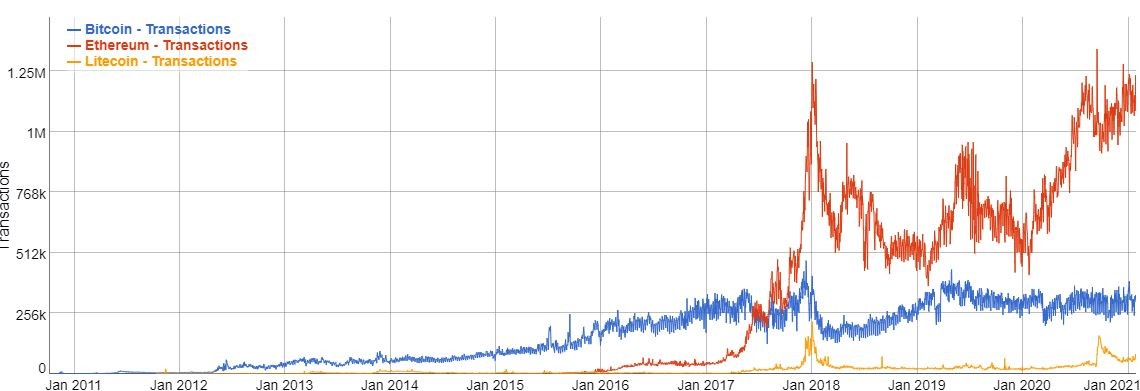
\includegraphics[scale=1]{assets/figures/blockchain_trend.jpg}
    \begin{flushleft}
        Quelle: Token S. 24
    \end{flushleft}
    \label{fig:birds8}
\end{figure}


\begin{figure}[!ht]
    \caption{Trend von Kryptowährungen}
    \includegraphics[scale=1]{assets/figures/investion blockchain solution.png}
    \begin{flushleft}
        Quelle: Token S. 24
    \end{flushleft}
    \label{fig:birds7}
\end{figure}


Ist der Trend begründet und wird sich die Technologie durchsetzten? Im Folgenden sollen nun beide Datenbanksysteme auf deren Wichtigste Kriterien untersucht werden.


\paragraphtitle{Kontrolle für Unternehmen}
Unternehmen benötigen einen bestimmten autoritativen Prozess, um die Blockchain-Technologie zu nutzen.
Anders als Big Data Anwendungen, werden öffentliche Blockchains nicht in der Lage sein, diese Kontrollmöglichkeiten in absehbarer Zeit zu bieten.
Der Aufstieg privater und konzerninterner Blockchains scheint jedoch sowohl die Kontrolle als auch den dezentralen Charakter der Technologie zu bieten. 
Diese werden meist als Enterprise-Blockchain-Frameworks bezeichnet und sind nur für Organisationen geeignet.


\paragraphtitle{Sicherheit}
„Sicherheit ist kein Vorteil oder Upgrade. Man erreicht sie nicht, indem man neue Schichten aus Passwörtern hinzufügt“. \footnote{google s 22}
Durch ihre grundlegende Funktionsweise, Transaktionen und Daten auf vielen Rechnern eines Systems zu verteilen, hat die Verschlüsselung bei Blockchains einen hohen Stellenwert. 
So würde beispielsweise der Angriff auf ein Bitcoin rund 30 millarden USD kosten.\footnote{\url https://gobitcoin.io/tools/cost-51-attack/}
Dies geschieht durch Umschreibung der Information in eine anscheinend zufällige Abfolge von Zeichen. Dies geschieht durch den sogenannten Schlüssel, welcher erforderlich ist, um die Information zu decodieren.
Anders als bei der Blockchain, vertritt Big Data den umgekehrten Ansatz. Die Idee hinter Big Data ist, dass die frühere langsame, unbeholfene, schrittweise vorgehende Suche nach Wissen durch menschliche Gehirne ersetzt werden kann, wenn zwei Bedingungen zutreffen: 
Alle Daten in der Welt können an einem einzigen Ort gesammelt werden und es können Algorithmen geschrieben werden, die hinreichend umfangreich sind, um sie zu analysieren.\footnote{google s 35}
Hier besteht oftmals die Gefahr, dass, sollte besagter Server offline gehen oder sogar kompromitiert werden, die Web-Applikation nicht zuverlässig ist.

\begin{figure}[!ht]
    \caption{Manipulation des Ledgers}
    \includegraphics[scale=1]{assets/figures/blockchange.png}
    \begin{flushleft}
        Quelle: Token S. 24
    \end{flushleft}
    \label{fig:birds2}
\end{figure}


\paragraphtitle{Fälschungssicher}
Ein Versuch, einen Block in der Blockchain zu manipulieren, würde den Hashwert dieses Blockes ändern, da sich der Inhalt ändert.\footnote{10xDna s 100}
Der sogenannte Konsensmechanismus ist ein Programm, das die einzelnen Knotenpunkte innerhalb einer Blockchain vergleicht und in der Lage ist, legitime Transaktionen erst zu identifizieren und dann der Blockchain hinzuzufügen.
Grund hierfür ist die Tatsache, dass jeder einen Block zur Blockchain hinzufügen kann, weswegen sichergestellt werden muss, dass keine falschen Informationen zu Elementen der Blockchain werden.
Des Weiteren sorgt er dafür, dass es eine allgemeine Übereinkunft der Daten innerhalb des Blockchain-Netzwerkes gibt, so dass die Verlässlichkeit dieser Daten gewährleistet wird.

\paragraphtitle{Kontrolle}
Wie bereits in der Einleitung erwähnt, war einer der ausschlaggebendsten Elemente der Web2-Epoche, dass die Nutzer auch die Rolle eines Produktes übernehmen. 
Das zeigt sich beispielsweise an der Sammlung von Nutzerinformationen, welche dann genutzt werden, um für jeden Nutzer spezifische Werbungen zu schicken, je nach seinen Vorlieben. 
Dies soll im Web3 mit Hilfe von Blockchain von Grund auf anders aufgebaut werden. Stichwort Basic Attention Token, kurz BAT. 
BAT ist ein System, welches in der Lage ist, die Aufmerksamkeit der Nutzer direkt zu belohnen. 
Somit wird die Rolle aller Akteure der Onlinewerbebranche neu definiert, wie auch die Beziehung zwischen Nutzern, Publicer und Werbetreibenden. 
Ziel dieser Idee ist, einen transparenteren und effizienteren Werbemarkt zu schaffen. BAT ist ein Token, welches von einer Public Blockchain verwaltet wird. 
Der Brave Browser hat eine integrierte Wallet, die zwei Tokens verwaltet: BAT, welches als Zahlungsmittel verwendet wird, und Basic Attention Metrics, das sicherstellt, dass die Aufmerksamkeit der Nutzer genau gemessen und berichtet wird. 
Werbetreibende senden diese BAT Tokens mitsamt den Werbeanzeigen verschlüsselt per Smart Contract. Sollte sich ein Nutzer dazu entscheiden, die Werbung anzusehen, kann er bis zu 70 Prozent der Werbeeinnahmen verdienen. 
Der Rest geht an den Webseitenbetreiber.

\paragraphtitle{Anonymität}
Bei Web2 Anwendungen findet die Nutzererkennung anhand der E-Mail-Adresse oder Benutzernamens zusätzlich des Passwortes statt.
Diese Informationen sind auf einem Server hinterlegt und werden geprüft, beispielsweise bei der Anmeldung. 
Bei der Blockchain hingegen findet dies durch den Private Key statt, welcher auf einem P2P verschlüsselt hinterlegt ist.
Durch die hohe Verschlüsselung, sowie durch die hinter Private Keys versteckte Anonymität gelten Blockchain Datenbanksysteme als Möglichkeit, unbekannt im Netz zu agieren.
Dies hat sich bereits als reale Gefahr dargestellt, da viele illegale Aktivitäten, insbesondere im Zahlungsverfahren heutzutage über Kryptowährungen, wie typischerweise Bitcoin, ablaufen.
Insbesondere, da diese Zahlungen nicht nachverfolgbar sind.
Der Betrag an Kryptowährung, der auf dem sogenannten Dark-Web-Marktplatz ausgegeben wurde, stieg in den letzten drei Monaten des Jahres 2019 um 60 Prozent auf einen neuen Höchststand von 601 Millionen US-Dollar, wie aus den am Dienstag veröffentlichten Daten von Chainalysis hervorgeht, einem Unternehmen, das alle Bitcoin-Transaktionen verfolgt und als Berater für mehrere Regierungsbehörden fungiert.\footnote{\url https://www.nytimes.com/2020/01/28/technology/bitcoin-black-market.html}

\begin{figure}[!ht]
    \caption{Bitcoin Wert im Darknet}
    \includegraphics[scale=0.7]{assets/figures/bitcoin_darkmarket.png}
    \begin{flushleft}
        Quelle: Token S. 19
    \end{flushleft}
    \label{fig:birds3}
\end{figure}

\paragraphtitle{Energieverbrauch}
Bei Big Data Netzwerken setzt sich der Energieverbrauch aus der durchgehenden Stromzufuhr des Servers und des Kühlsystems zusammen, was zu hohen Energiekosten für das Unternehmen führt. 
Bestimmte Blockchain-Konsensmechanismen haben jedoch höhere Energiekosten.
Wie bereits angemerkt muss ein Konsensprozess durchgeführt werden, um sicherzustellen, dass jede Transaktion gültig ist. 
Es liegt auf der Hand, dass der Konsensprozess einen enormen Aufwand für die Bildung jedes Knotens erfordert. 
Ganz zu schweigen davon, dass alle Knoten hin und her kommunizieren müssen, um sicherzustellen, dass eine Transaktion gültig ist.
Blockchain-Netzwerke wie Bitcoin verwerden hierbei den Proof of Work, bei welchem jeder Node eine mathematische Funktion löst. 
Der erste, der die Lösung der Funktion findet, bekommt als Belohnung Bitcoins.
Es gibt aber auch andere Konsensmechanismen, bei denen der Energieverbrauch deutlich geringer ist, so beispielsweise der Proof of Stake.
Anders als bei den Proof of Work, wird bei dem Proof of Stake gelost. 
Der Gewinner, auch Validator genannt, überprüft den nächsten Block und alle darin aufgezeichneten Transaktionen. 
Um an diesem Losverfahren teilzunehmen, müssen die Knoten, die als Validator fungieren wollen, eine bestimmte Anzahl von Coins in das Netz einbringen, was im Grunde als Garantie fungiert. 
Je höher die Anzahl der Coins, der sogenannten Stake, desto höher ist die Wahrscheinlichkeit, als Validator ausgewählt zu werden. 
Die als Garantie hinterlegten Coins garantieren auch, dass der Prüfer keine betrügerischen Transaktionen akzeptiert: tut er dies doch, verliert er einen Teil seines Stakes. 
Als Belohnung für die Überprüfung erhält der Überprüfer in der Regel eine Transaktionsgebühr in Form eines Tokens des jeweiligen Netzwerkes.\footnote{10xdna s }

\begin{figure}[!ht]
    \caption{Energieverbrauch PoW vs PoS}
    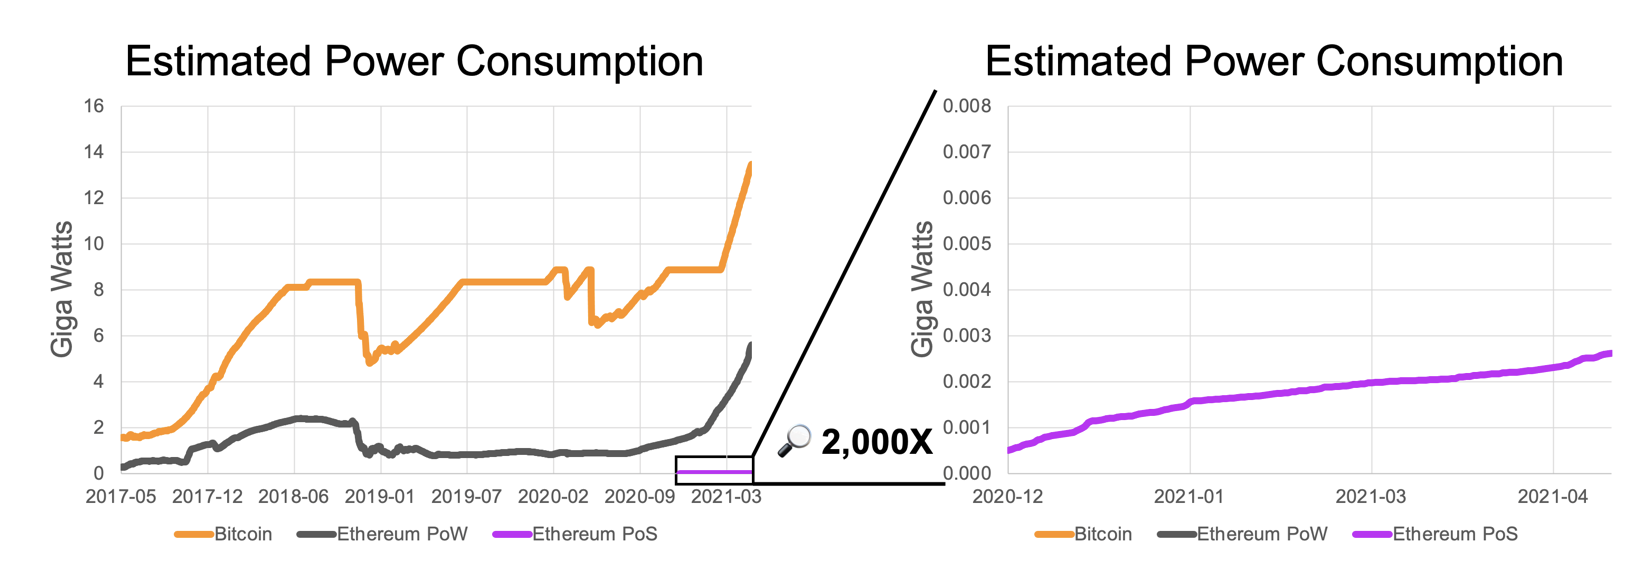
\includegraphics[scale=0.6]{assets/figures/power_consumption.jpg}
    \begin{flushleft}
        Quelle: Token S. 19
    \end{flushleft}
    \label{fig:birds4}
\end{figure}

\paragraphtitle{Preis}
Zusätzlich zu den Energiekosten fallen noch weitere Gebühren an wie Hardware, Infrastruktur und Personal.
Bei einem dezentralen Netzwerk werden diese Dienstleistungen outsourced auf Freiwilligenbasis der Nutzer.

%FAZIT---------------------------------------------%
\subsection{Gründe für die Wahl der Hypothese}
Wie aus dem vorherigen Kapitel zu entnehmen ist, bieten sowohl BigData als auch Blockchainsysteme viele verschiedene Vor- und Nachteile für Internetdienstleister. 
Dezentrale Systeme haben die letzten Jahrzehnte stark geprägt und den Weg für viele neue Ideen und Systeme eröffnet.
Es gibt immer mehr Skandale in punkto Datenraub oder Intransparenz zentraler Webseitenbetreiber, was die allgemeine Nachfrage nach neuen, sichereren Alternativen steigen lässt. 
Zusammen mit der sich verbessernden Technologien und den oben genannten Vorteilen lohnt es sich für viele Unternehmen, schon heute auf Blockchain umzusteigen.
Selbst wenn es ein eher langwieriger Prozess wird, wären vermutlich zehn Jahre ein denkbares Zeitfenster, um besagtes Ziel zu erreichen.



%FAZIT---------------------------------------------%
\subsection{Argumentation}


\subsubsection{Umsetzbarkeit}
Da die zugrundeliegende Technologie dafür schon gegeben ist, wäre die Frage vielmehr, ob es sich für Unternehmen lohnt.
BitTorrent, Popcorn Time, BitMessage und Tor sind allesamt dezentrale Anwendungen, die von einem PHP-Netzwerk verwaltet werden, das kein Blockchain-Netzwerk ist. 
Blockchain- Netzwerke sind eine verbesserte Form von P2P-Netzwerken. Näheres dazu wird unten im Anhang unter „Geschichte von Bitcoin und dem Web3“ erklärt.

\paragraphtitle{Public/Private Blockchain}
Der Unterschied zwischen einer Public und einer Private Blockchain liegt darin, wer Mitglied des Netzwerks sein und die Konsensmechanismen ausführen darf. 
Jeder, der die im Protokoll festgelegten Regeln und Verfahren befolgt, kann einem öffentlichen Blockchain- Netzwerk  beitreten.  
Bitcoin  zum  Beispiel  ist  ein öffentliches Blockchain-Netzwerk.
Im Gegensatz dazu ist ein privates Blockchain-Netzwerk geschlossen. 
Private Netzwerke können nur per Einladung beigetreten werden. 
Mitglieder müssen nach bestimmten Regeln validiert werden. Hier wird bestimmt, wer was sehen kann und wer an welchen Transaktionen teilnehmen darf. 
Private Blockchains werden in der Regel von Unternehmen oder Regierungen betrieben, dabei können sich u. U. Einzelpersonen oder Organisationen daran beteiligen.

\paragraph*{\mbox{}}
Da außerdem die meisten Unternehmen bereits über ein zentrales Datenbanksystem verfügen, müssten sie für die entstehenden Kosten eines Wechsels aufkommen.
Man beachte hierbei, dass es aufgrund der Tatsache, dass die dazu erforderliche Technologie ein relativ wenig verbreitetes Konzept ist, nicht viele fähige Entwickler gibt, die daran arbeiten können. 
Wenn Unternehmen also versuchen, ihre Blockchain-Lösung für den eigenen Betrieb zu entwickeln, kann es u. U. schwierig werden, ein fähiges Team fürs Projekt zu finden. 
Blockchain ist nicht für Unternehmen gedacht, die Legacy-Netzwerke (ältere Systeme) betreiben. 
In Wirklichkeit würde die Blockchain die alten Netze ersetzen. 
Allerdings ist der Integrationsprozess noch nicht voll funktionsfähig. 
Außerdem sind viele Blockchain-Technologien nicht in der Lage, mit den alten Netzen zusammenzuarbeiten. 
Das bedeutet, dass die Unternehmen, um sie richtig nutzen zu können, ihre alten Netze endgültig abschaffen müssten. 
Diesem Umstand stehen viele skeptisch gegenüber.


\subsubsection{Zukunftstauglichkeit}
Das Internet hat sich in den letzten Jahren zu einem Einkaufsladen für Benutzerinformationen verwandelt, von welchem die Nutzer kaum profitieren.
P2P-Netzwerke wie Blockchain versprechen hier Anonymität, Kontrolle und Sicherheit und vor allem weniger Abhängigkeit von Unternehmen.

Wir überschätzen immer die Veränderungen, die in den nächsten beiden Jahren passieren sollen. Aber wir unterschätzen den Wandel, der über die nächsten zehn Jahre passiert. Lass’ dich dadurch nicht zur Untätigkeit verleiten. Bill Gates

Wie bereits festgestellt existiert bereits eine vielversprechende Technologie dazu. 
Im letzten Jahrzehnt kam es zu hunderten Skandalen von Big-Data-Unternehmen aufgrund ihrer teilweise fragwürdigen Strategien, Profit zu erzielen. 
Auf Blockchain basierende Seiten bieten hingegen eine höhere Transparenz, sowie die Möglichkeit für Nutzer, sich an diesem Prozess finanziell selbst zu bereichern.
Auch wenn die Technologie von Blockchain Netzwerken und der gesetzliche Rahmen dazu noch nicht ausgereift ist, besagt der Trend, dass wir damit zu rechnen haben, zumal es bereits funktionierende Geschäftsmodelle und Währungen gibt.
Viele Tech-Führungskräfte und Ingenieure haben bereits große IT-Unternehmen wie Google, Meta und Amazon verlassen, um die ihrer Meinung nach einmalige Chance der Kryptowährung zu nutzen.\footnote{\url https://www.nytimes.com/2021/12/20/technology/silicon-valley-cryptocurrency-start-ups.html?searchResultPosition=4}
%FAZIT---------------------------------------------%
\subsection{Fazit}
Auch wenn wir uns mittlerweile auf die Zuverlässigkeit unzähliger Dienste verlassen, laufen im Hintergrund Datenbanken, welche im Kern wenig Sicherheit gewährleisten können. 
Unberechtigte Zugriffe sind möglich und können nicht immer verfolgt werden. DLTs ändern das, und so sind sie denkbar eine Technologie fürs kommende Zeitalter. 
Verschlüsselung, Speicherung, Validierung und Sicherung der Daten funktionieren hier in einer integrierten Lösung. 
Alle Daten, denen wir vertrauen müssen, werden in Zukunft in einem Distributed Ledger bzw. einer Blockchain gespeichert werden. Neue Geschäftsmodelle können entstehen – direkt zwischen Nutzern und Anbietern, ohne Mittelsmänner. 
Es ist allerdings auch zu bedenken, dass herkömmliche Datenbanken deutlich effizienter, einfacher und günstiger zu betreiben sind.
Überall dort, wo wir die Sicherheit der Blockchain oder Funktionen wie Smart Contracts nicht brauchen, sind sie daher weiterhin die bessere Wahl.